%!TEX root = ../thesis.tex
\chapter{Multi-speaker text-to-speech modeling} \label{ch:tts}
\section{Overview}
Text-to-speech systems recently achieved almost indistinguishable quality from human speech. However, the prosody of those systems is generally flatter than natural speech, producing samples with low expressiveness. Disentanglement of speaker id and prosody is crucial in speech generation systems to improve on naturalness and produce more variable syntheses \autocite{markovi2015}. 

This chapter proposes a new neural text-to-speech model that approaches the disentanglement problem by conditioning a \textit{Tacotron2}-like architecture on flow-normalized speaker embeddings, and by substituting the reference encoder with a new learned latent distribution responsible for modeling the prosody-driven variability. By removing the reference encoder dependency, not only the speaker-leakage problem typically happening in this kind of systems disappears, producing more variable syntheses at inference time, but the system becomes much more lightweight, not depending on a production TTS system to be executed. This is a first step that enables low-resource on-device offline execution The new model achieves significantly higher prosody variance than the baseline in a set of quantitative prosody features, as well as higher speaker distinctiveness, without decreasing the speaker intelligibility. Finally, the normalized speaker embeddings enable much richer speaker interpolations, substantially improving the distinctiveness of the new interpolated speakers.

 %This research study has been conducted as part of the author's work at \textit{Alexa AI}, and has already been published in the proceedings of the \textit{Interspeech} conference of 2021 \autocite{valles2021b}.

\section{Introduction}
In the last five years speech technologies have improved considerably. The text-to-speech (TTS hereafter) field has been largely benefited by the rise of deep learning \autocite{Sisman2021}, which allowed these systems to achieve near-human performance at synthesizing speech that is almost indistinguishable from human's. One of the first achievements was \textit{WaveNet} \autocite{vanderoord2016}, a neural vocoder based on dilated causal convolutions that was able to surpass its predecessors in naturalness in 2016. With the rise of the attention mechanism and its variants \autocite{bahdanau2015,vaswani2017,chaudhari2019}, \textit{Tacotron} \autocite{Wang2017} and \textit{Tacotron 2} \autocite{Shen2018,liu2019b} proposed a sequence-to-sequence architecture as an end-to-end TTS solution. These models were able to map input text (or phonemes) to a spectrogram that, given the right neural vocoder (\textit{WaveNet} for instance), would be converted into a sequence of waveform samples.

TTS is fundamentally a generative modeling problem because a given sentence can be mapped to multiple utterances with different prosody and speaker characteristics \autocite{Taylor2009}. \textit{Tacotron}, in its initial form, is a supervised model that performs a hard mapping between the input text and the output spectrograms. Therefore, the utterances generated using \textit{Tacotron}-like architectures, although natural, they follow the average prosody of the training set, not allowing to generate utterances of a sentence with multiple speaking styles.

\section{Previous work}
The authors of \autocite{skerryryan2018} attempt to remediate the lack of expressiveness of the model by introducing a reference encoder consisting of a latent distribution that is conditioned on a reference mel-spectrogram (usually the target spectrogram, at training time). This distribution is learned by the model through a bottleneck that is intended to capture prosody aspects of the target spectrogram, preventing phonetic or speaker information to flow through. In practice, specially when using this approach in multi-speaker settings, the model tends to leak speaker information to the output. This represents a problem at inference time, when a synthetic neutral reference is provided (generally synthesized using a production system similar to \textit{Amazon Polly}), given that the synthesized speaker identity tends to resemble the reference instead of the target voice. This problem is known as speaker leakage and it was already reported in \autocite{skerryryan2018}, where the authors emphasize the importance of properly tuning the size of the reference bottleneck to amend it. In addition, the usual dependence of this model in a production TTS system makes them unfeasible for low resource, on-device or offline implementations, besides their obvious negative impact in energy efficiency.

In \autocite{liu2020c}, the authors propose using a multi-task version of \textit{Tacotron} to enhance the prosody of the syntheses. The approach described in the paper consists of jointly learning the target mel-spectrogram as well as the probability distribution of the phrase break patterns for each word. The work of \autocite{liu2020c} proposes a novel training schema for \textit{Tacotron} where deep style features are extracted using the \textit{SER} framework (\autocite{Zhang2018, Lotfian2019}). These features are later used for minimizing the style differences between the real and synthesized samples.

This chapter's contribution builds upon a multi-speaker \textit{Tacotron} architecture with a reference encoder (similar to \autocite{skerryryan2018}) and propose two modifications: (1) replaces the pre-trained speaker embedding with a normalized speaker embedding using normalizing flows \autocite{kingma2018}, that allows sampling from the learned \textit{Gaussian} distribution and (2)  substitutes the reference encoder with a residual encoder, which learns a latent distribution conditioned on the input phonetic information, allowing the model to capture and encode the residual attributes not present in the linguistic input and the speaker embedding.

Inspired by the work of \autocite{Raitio2020}, the proposed model achieves significantly higher prosody variation by measuring the difference in variance between the baseline and the proposed model across a set of features derived from the fundamental frequency, the energy, the signal to noise ratio and the speaking rate. These features capture most of the prosody variables (pitch, speed, loudness and timbre) \autocite{Raitio2020} and allow performing objective comparisons between systems.

%The contribution can be summarized in the following points: (1) proposal of a new architecture that significantly increases the prosody variability of the syntheses with no intelligibility and distinctiveness degradation, (2) the proposed architecture removes the dependency on a production voice system as it does not use a reference spectrogram, which makes it more computational efficient, (3) when interpolating between speaker embeddings the synthetic speakers from the proposed model are significantly more distinct than the ones of the baseline.

\section{Methods}
A \textit{Tacotron2}-based sequence-to-sequence model with \textit{location-based attention} \autocite{Wang2017} is used as a baseline throughout this study. This baseline architecture is represented in figure \ref{fig:architectures}-top. A couple of encoder branches are added over the initial \textit{Tacotron} architecture to allow the model to synthesize multiple speakers: the speaker branch and the reference branch. The first one takes as input a pre-trained speaker embedding vector representing the speaker characteristics. This vector is obtained from the output of a speaker verification model trained to minimize a triplet loss. This speaker verification model is pre-trained using pairs of utterances, similar to  \autocite{Ren2019}. For every speaker, the vectors corresponding to all their utterances are pre-computed and then averaged to form the speaker vectors. As a result, a fixed size vector is produced for every speaker in the dataset. Additionally, the proposed architecture includes a reference branch that is conditioned on the target spectrogram (at training time) and is intended to learn a latent distribution summarizing the prosody information, similar to the proposal of \autocite{skerryryan2018}.




The proposed architecture builds upon the baseline model, removing the dependency of the reference branch on the target spectrogram, because it tends to cause speaker/phonetic leakage (read the section 4 of the samples included in \autocite{skerryryan2018}). It also slows down the inference process as it requires a production TTS system to provide the references. Instead, a learnable variational latent space conditioned on the phonetic information is learned together with a set of learnable free parameters (named \textit{residual branch}). The purpose of this branch is to encode the prosody information not present in the input linguistic features or in the speaker embedding vector in a new latent space (i.e. the residual prosody variance). Moreover, the speaker embedding vectors are normalized using normalizing flows based on the work of \autocite{kingma2018}, so that the normalized vectors follow a \textit{Gaussian} distribution. That change enables sampling from the speaker embedding latent space instead of just using the average embedding vector. This increases the coverage of the speaker embedding space, allowing smoother interpolations between speaker embedding vectors. The architecture proposed is depicted in figure \ref{fig:architectures}-bottom

% TODO: \usepackage{graphicx} required
\begin{figure}[h!]
	\centering

	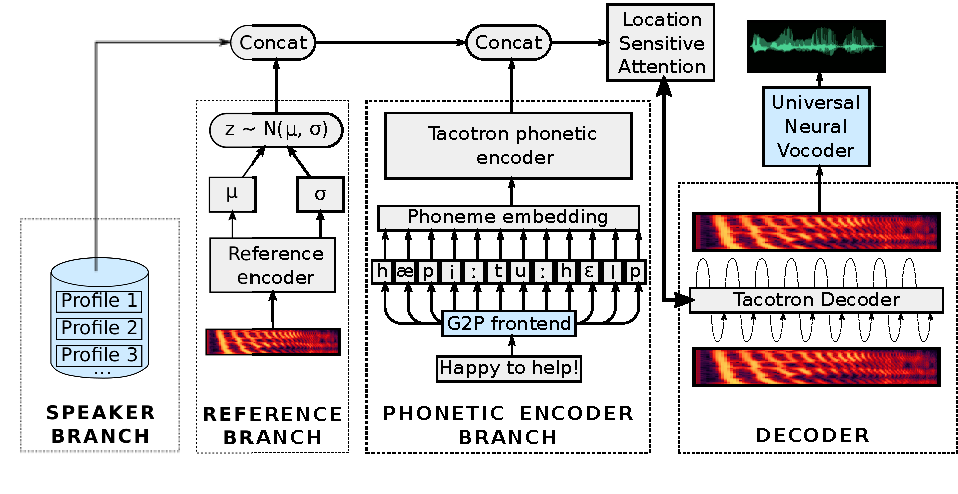
\includegraphics[width=1.0\linewidth]{tts/images/baseline_architecture}

	\vspace{0.5cm}

	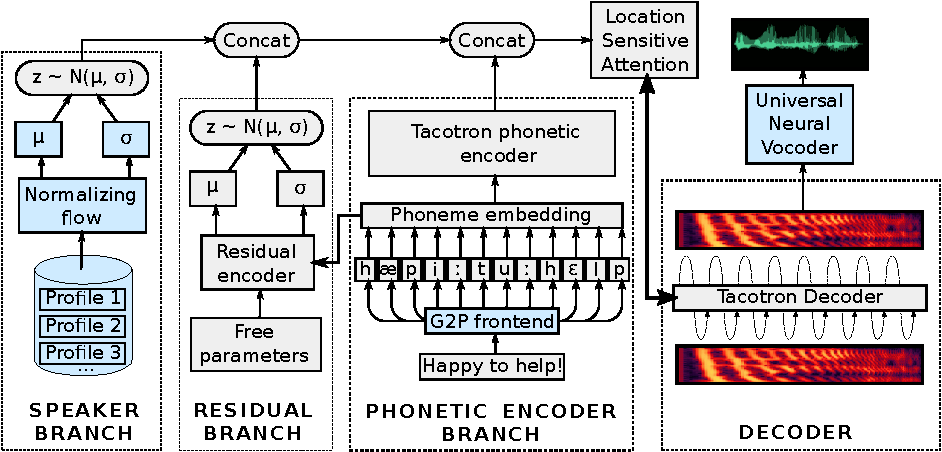
\includegraphics[width=1.0\linewidth]{tts/images/proposed_architecture}

	\caption[TTS baseline vs proposed architectures]{Top: the baseline architecture. Bottom: the proposed architecture. The blue blocks represent pre-trained parts of the network and the blocks with round corners are tensor operations.}
	\label{fig:architectures}
\end{figure}


\subsection{Speaker embedding normalization with flows}
Normalizing flows \autocite{rezende2015} are powerful methods for producing tractable distributions from which one can sample. Through a sequence of invertible functions (named flows) they transform a complex data distribution to a tractable probability distribution. The output distribution is usually chosen to be an isotropic unit \textit{Gaussian} (with mean 0 and variance 1) to allow for smooth interpolations and efficient sampling. A more detailed description of these models is given in chapter \ref{sec:flows}.

\textit{Glow} \autocite{kingma2018}, a flow-based generative model, has shown significant improvements in computer vision generative modeling by adding invertible 1x1 convolutions to the sequence of transformations applied to the input. To train this model on one-dimensional speaker embedding vectors, the 2-dimensional convolutions from the original architecture, designed for computer vision tasks, have been replaced with 1-dimensional ones.

A normalizing flow has been trained to normalize the pre-trained speaker embeddings described previously. The trained model attains a \textit{Gaussian} distributed latent space of speaker embeddings from which one can easily sample to create embeddings representing new, unseen speakers. The proposed architecture samples speaker representations from the \textit{Gaussian} distribution defined by the normalized embeddings, both at training time and at inference time.


\subsection{Residual branch}
The new residual branch is designed with the idea of giving the model the capability to learn the prosody-induced variance that cannot be explained by the linguistic features and the speaker embedding vector alone. It takes as input the linguistic features and a set of learnable free parameters\footnote{Notice that the dense layers that produce the residual latent distribution parameters do not have bias terms, so that all the bias is learned in the free parameters vector.}, conditioning on the target sentence and on a global prior. The motivation behind this design is to help the network learn different ways of uttering a given input sentence (linguistic features conditioning), and the potential global biases existing in the training dataset (free parameters).

The output of the phonetic encoder $\mathbf{h_{\text{ph}}}$ is piped into a bidirectional recurrent neural network \autocite{schuster1997,graves2005} in order to get a representation independent of time. The last output of the recurrent neural network of both, forward and reverse passes (represented in equations \ref{eq:rnn1} and \ref{eq:rnn2} as $\mathbf{o_f}$ and $\mathbf{o_r}$, respectively), are  concatenated to form a fixed-size phonetic representation $[\mathbf{o_f}, \mathbf{o_r}]$. 

The joined output vector of the bidirectional \textit{RNN} stage is concatenated with a vector of free parameters $\mathbf{v_f}$ and the result is passed through two stacked dense layers to form the parameters of the residual latent distribution (as shown in equation \ref{eq:residual}, where $g$ represents the \textit{ReLU} activation function). The $h_{residual}$ vector is split in two vectors $h_{residual}^{\mu}$ and $h_{residual}^{\sigma}$ from where a latent vector $z$ is sampled using the re-parametrization trick \autocite{kingma2019}. 

Finally, a \textit{Kullback-Leibler} divergence loss is included to assure that the distribution of the latent representation approximates an isotropic \textit{Gaussian} distribution.

\begin{equation}
 \label{eq:rnn1}
\mathbf{o_f} = \text{RNN}_f(\mathbf{h_{ph}})
\end{equation}

\begin{equation}
 \label{eq:rnn2}
\mathbf{o_r} = \text{RNN}_r(\mathbf{h_{ph}})
\end{equation}

\begin{equation}
 \label{eq:residual}
\mathbf{h_{residual}} = \mathbf{W_2}(g(\mathbf{W_1}\cdot([\mathbf{o_f}, \mathbf{o_r}, \mathbf{v_f}]) + \mathbf{b1} )) +\mathbf{ b_2}
\end{equation}

\section{Experiments and results}
\subsection{Setup}
 A combination of two internal datasets is used to train the models, one of them containing 2860 non-professional speakers, with 200 utterances per speaker on average, and the other containing 10 professional speakers, with 13,000 studio-recorded utterances per speaker – totaling to 2870 speakers and more than 700,000 utterances. The audio utterances are downsampled at 16kHz and 80 dimensional mel-spectrograms are extracted. The frame width is defined as a $50ms$ window, with an overlap of $12.5ms$. A universal neural vocoder is used to synthesize the wav samples \autocite{lorenzotrueba2019}. The linguistic features have been extracted using a proprietary internal front-end which takes the text as input and extracts the phonemes, that are used as input for the model. The speaker embedding, the free parameters and the residual distribution parameters $\mu$ and $\sigma$ vectors were defined to have a length of 192 elements.

 The models have been trained for one million steps, with a mini-batch size of 24. Then 50 unseen sentences are synthesized with each of the 2870 speakers voices. The syntheses have been evaluated in 3 ways: intelligibility, distinctiveness and prosody variability.

 Additionally, 50 speakers are randomly sampled from the pool of 2870 speakers and generated interpolations (linear) between all the possible pairs, in order to study how the proposed model and the baseline behave in this setting.

 \subsection{Intelligibility}
\textit{AWS transcribe} system is used to transcribe each of the syntheses, and then measure the word error rate (\textit{WER}) between the target sentence and the transcription \autocite{uday2019}. These metrics are aggregated as the average \textit{WER} per speaker. A median word error rate of $8.5\%$ is achieved in the baseline, while a $8.3\%$ WER is achieved by the proposed architecture. Although significative, this difference is very small, concluding that both models are roughly equivalent in terms of intelligibility.


% TODO: \usepackage{graphicx} required
\begin{figure}[h]
	\centering
	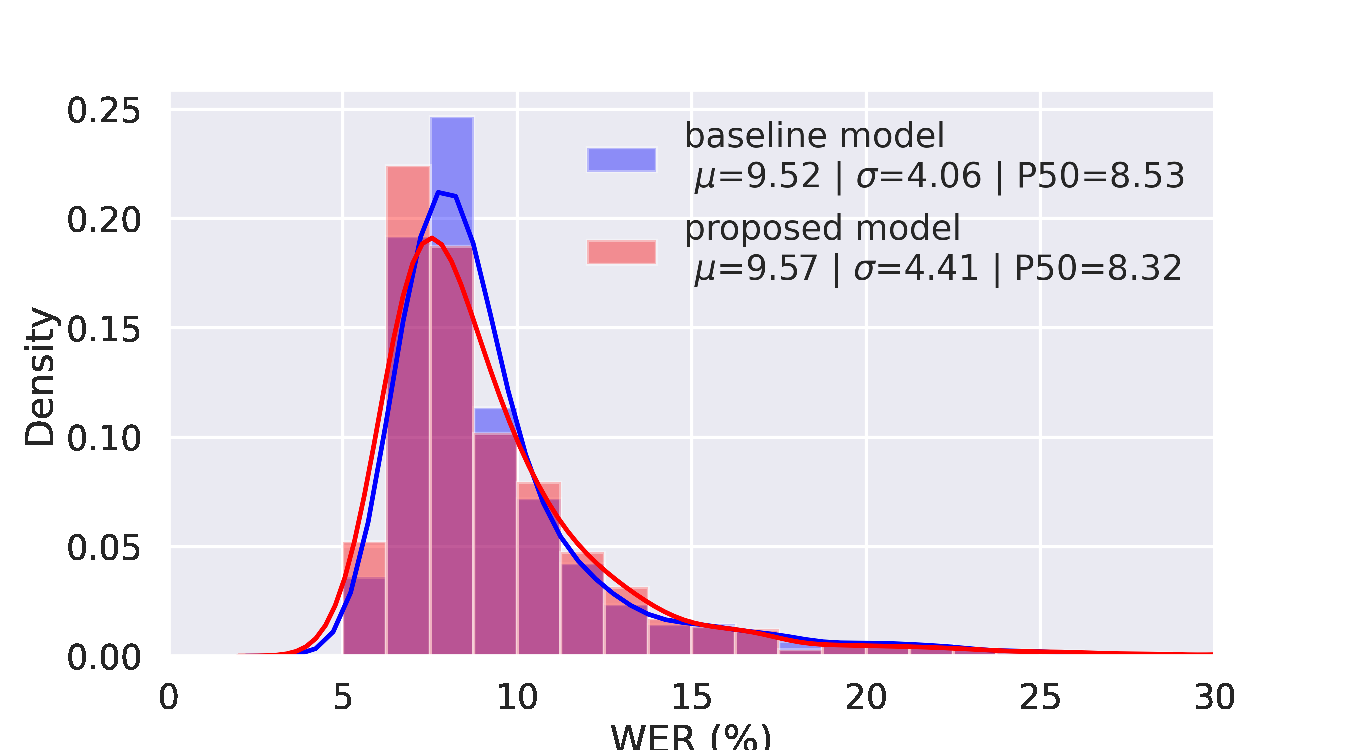
\includegraphics[width=0.7\linewidth]{tts/images/wer}
	\caption[Speaker intelligibility curves for the TTS models]{Speaker intelligibility of the baseline and proposed models, measured as word error rate of the target and the transcribed synthesis, showing a slightly smaller error for the proposed architecture (Wilcoxon's $p=0.0305$). The solid lines represent a kernel density estimate (KDE) over the histograms.}
	\label{fig:wer}
\end{figure}


\subsection{Distinctiveness}
To measure how distinct the synthesized speakers are, \textit{Alexa}'s internal \textit{speaker verification system} is used.  Each utterance is compared with 4 samples randomly drawn from the full pool of samples. The false acceptance rate (\textit{FAR}) is used as a metric to quantify the percentage of speaker pairs incorrectly identified as the same speakers by the speaker verification model. Equation \ref{eq:far} shows how \textit{FAR} is computed in detail, where $\mathcal{C}(i)$ is 1 if the $i$th pair of samples is misclassified as different speakers and $N$ is the total number of pairs in the pool. Figure \ref{fig:far} shows how the \textit{FAR} metric varies for both, the proposed model and the baseline as the classification threshold varies. Table \ref{tab:far} shows the \textit{FAR} score for four arbitrarily picked thresholds. Lower values of \textit{FAR} mean higher distinctiveness.

\begin{equation}
    FAR = \frac{1}{N}\sum_{i=1}^{N} \mathcal{C}(i)
    \label{eq:far}
\end{equation}


\begin{figure}[h]
	\centering
	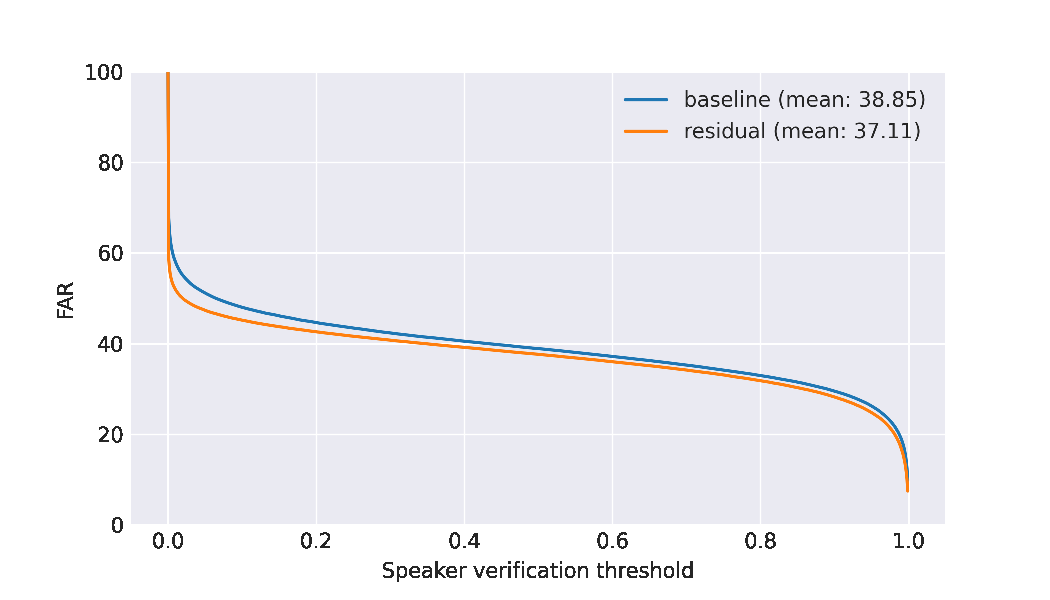
\includegraphics[width=.7\linewidth]{tts/images/far}
	\caption[False acceptance rates for the TTS models]{false acceptance rate distribution at different \textit{speaker verification model} thresholds.}
	\label{fig:far}
\end{figure}

\begin{table}[h]
	\centering
	\caption[False acceptance rates for different thresholds of the TTS models]{false acceptance rate metric for different thresholds}
	\footnotesize
	\begin{tabular}{ccc}
		\toprule
		\textbf{Threshold} & \textbf{FAR-Baseline model} & \textbf{FAR-Proposed model} \\
		\midrule
		85\% & 31.49\% & 30.27\% \\

		90\% & 29.50\% & 28.21\% \\

		95\% & 26.23\% & 24.77\% \\

		99\% & 19.05\% & 16.93\% \\
		\bottomrule
	\end{tabular}
	\label{tab:far}
\end{table}



\subsection{Prosody variability}
To measure how much prosody and quality variability the new model introduces with respect to the baseline, a set of objective metrics has been defined inspired on the work of \autocite{Raitio2020}. Those metrics are listed in table \ref{tab:metrics}.

\begin{table*}[h!]
	\scriptsize
		\centering
	\caption[Summary of prosody variability metrics for TTS models]{Metrics used to quantify the prosody variation and quality across different models.}
	\begin{tabular}{p{0.3\textwidth}|p{0.7\textwidth}}
		\toprule
		Metric & Description \\
		\midrule
		f0 mean &  Mean of the fundamental frequency (calculated using SPTK \autocite{sptk} considering only the vocal sounds (non-zero components), with frame skip of 12.5ms.\\
		f0 range & Difference between the 5th and 95th percentiles of f0. \\
		speaking rate & Calculated as the number of phonemes in the sentence divided by total duration of the synthesis. \\
		f0 slope & Calculated as the slope of a linear fit using least squares in the f0 trajectory. \\
		snr & Signal to noise ratio calculated using SOX \autocite{SOX} as the difference in RMS dBs between the loudest and the quietest windows, using windows size of 50ms. \\
		power mean & $20\log10(\hat{x})$, where $\hat{x}$ is the average absolute amplitude with frame skip of 12.5ms. Only considering the vocal sounds. \\
		power range & Difference between the 5th and 95th percentiles of the power along time. \\
		power slope & Calculated as the slope of a linear fit using least squares in the power plot. \\
		\bottomrule
	\end{tabular}
	\label{tab:metrics}
\end{table*}



For this experiment, 50 speakers and 50 sentences have been picked. Then, 30 samples have been synthesized for every speaker-sentence pair varying the random seed, so different latent vectors are drawn from the latent distributions in each repetition. This procedure is repeated four times: (1) with the baseline model, (2) with the proposed model multiplying the $\sigma$ parameter of the speaker embedding distribution by zero (so that the latent vector becomes the mean of the speaker embedding latent distribution), (3) with the proposed model multiplying the $\sigma$ parameter of the residual distribution by zero, and (4) allowing sampling from both branches in the proposed model. Then the following comparisons are performed: the syntheses of (1) vs (2), (1) vs (3) and (1) vs (4) .

For the comparison, as the focus of this study is to measure differences of variance for the variables defined in the table, the \textit{bootstraping} technique is used to approximate the variance distribution for every variable in every speaker-sentence pair, and then a one-way \textit{Wilcoxon Signed-Rank} sum test between the groups is conducted. A significance level of $\alpha=5\%$ is used, over which the \textit{Bonferroni} correction ($\alpha=0.05/2500=0.002\%$) is applied. The results of the tests are summarized in the figure \ref{fig:wilcoxon}.

% TODO: \usepackage{graphicx} required
\begin{figure}[h!]
	\centering
	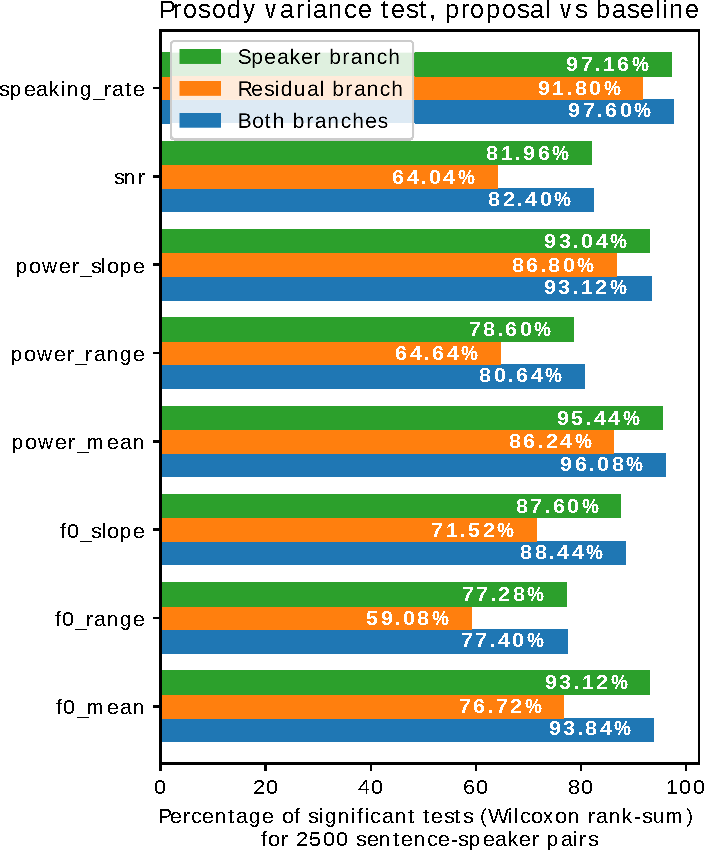
\includegraphics[width=0.7\linewidth]{tts/images/wilcoxon}
	\caption[Comparison of prosody variability between TTS models]{Baseline model vs proposed model when sampling from the residual latent distribution (blue) or from the speaker embedding distribution (orange), keeping the other constant. The results are represented as proportion of speaker-sentence pairs for which the proposed model shows significantly higher variance than the baseline, for each of the previously defined prosody features.}
	\label{fig:wilcoxon}
\end{figure}

Informal listening tests of the syntheses confirm that when sampling from the residual distribution (keeping the speaker embedding distribution constant), the variations in the syntheses are related with prosody aspects like the speaking rate, syllable duration or intonation, keeping the speaker identity untouched. When sampling from the speaker embedding distribution, small variations on the speaker identity are noticed.



\subsection{Speakers interpolation}
The proposed model and the baseline are tested using interpolated speakers to study how the speaker embedding normalization affects the intelligibility and distinctiveness of the new speakers. For that, 50 speakers have been chosen. All the pairs of speakers have been interpolated using linear interpolation, generating 1225 new voice profiles. Fifty sentences have been synthesized using those new voices and then evaluated distinctiveness and intelligibility (results in figure \ref{fig:svps}).

% TODO: \usepackage{graphicx} required
\begin{figure}[h!]
	\centering
	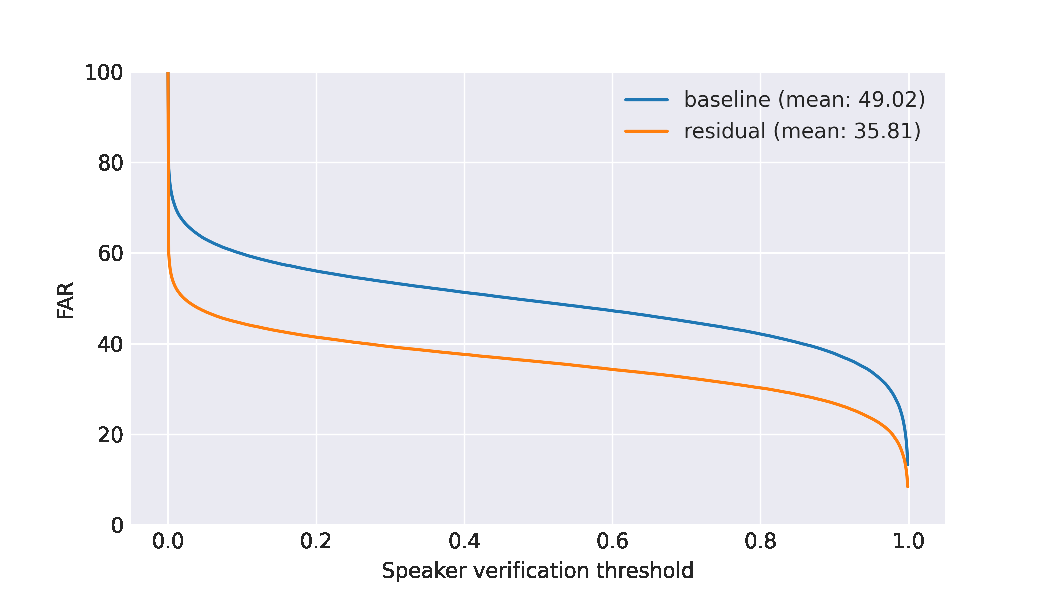
\includegraphics[width=0.7\linewidth]{tts/images/far_svps}

	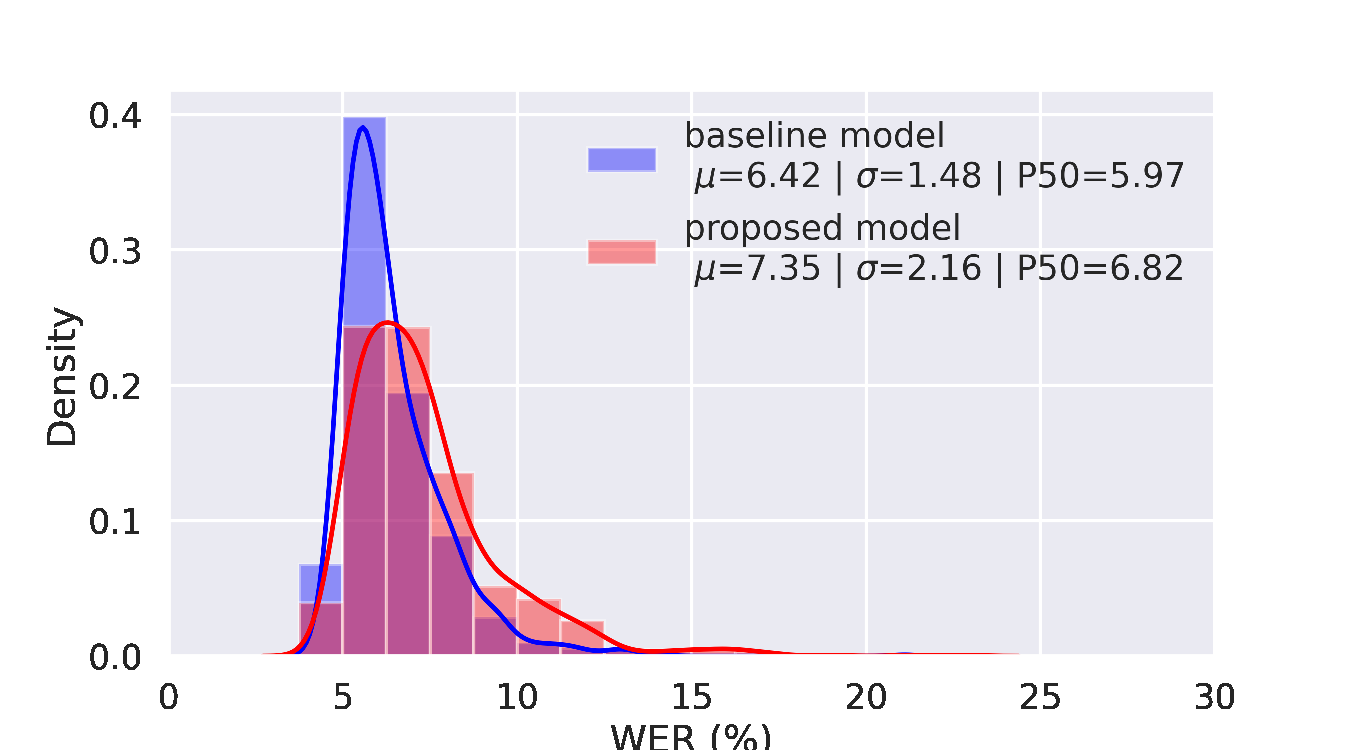
\includegraphics[width=0.7\linewidth]{tts/images/wer_svps}
	\caption[Speaker interpolation results for the TTS models]{Top: false acceptance rate distribution at different speaker verification thresholds, for all the interpolated speakers. Bottom: speaker intelligibility of the baseline and residual models, measured as word error rate of the target and the transcribed synthesis, showing a slightly smaller error for the baseline architecture (Wilcoxon's $p=5.2263\cdot 10^{-6}$). The solid lines represent a KDE over the histograms.}
	\label{fig:svps}
\end{figure}

The proposed model achieves 13.11\% lower FAR than the baseline. The rationale behind this is that the normalized speaker embedding space has a denser latent distribution than the one in the baseline. Given that the proposed model is trained on samples drawn from the normalized speaker embedding distribution (as opposed of using average vectors as in the baseline model), the denser latent space leads to a better generalization.


From the intelligibility perspective, the baseline shows an average WER of $6.42\%$ while the proposed model achieved a $7.35\%$. That difference is attributed to the fact that the interpolated speakers in the baseline are less distinctive and resemble much more to one of the two actual speakers, hence its intelligibility is naturally higher at the cost of a worse distinctiveness. Although significative, the difference in practice is negligible.


\section{Conclusions}


This chapter presents a new TTS architecture that allows increasing the prosody variance of a multi-speaker TTS system by learning the residual prosody into a new latent distribution. 

It has been also showed that by sampling from the residual and normalized speaker latent distribution the model produces syntheses with significantly different prosodies as measured by a set of quantitative metrics. The inclusion of the residual distribution also enables removing the reference spectrogram dependency. This does not only allow for a faster and  cheaper inference, but also solves potential speaker leakage issues, given that the model does no longer depend on a voice production system to work.


Finally, the normalization of the speaker embedding latent space allows for better speaker interpolation when compared with the baseline model, thus producing more diverse and unseen synthetic speakers.


